\section{Results} 

\subsection{Fixed versus variable force field} \label{first_phase}

The experimental results are summarized in Fig. \ref{figTC}, 
where the absolute mean errors (defined as absolute difference between the arrival point of the ball and the corresponding position of the paddle) are shown for the two conditions \textit{Test} and \textit{Control}.

\begin{figure}[tbp]
	\centering
		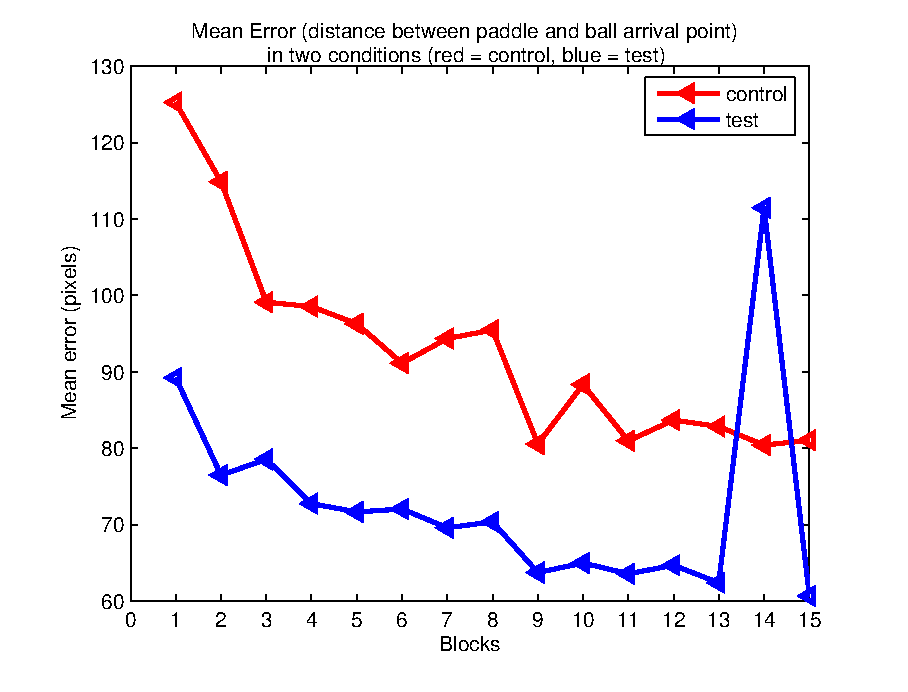
\includegraphics [width=15cm] {fig/TC.eps}
	\caption{Absolute mean error (absolute difference between paddle and ball arrival point) in the two conditions (red = control, blue = test)}
	\label{figTC}
\end{figure}

The two trends appear to be well separated; in particular the latter presents a larger error during the whole experiment, with the exception of the 14th block, in which we observe a sudden error increase in the \textit{Test} condition. After this block, \textit{Test}'s error return to a value in trend with the preceding blocks. We call this particular error variation \textit{Transfer Effect}. In both conditions a gradual error decrease appears from block to block, that could suggest the existence of a common progressive learning, due, for instance to an increasing skill in using the experimental setup.
These qualitative observation are supported by statistical analysis. An ANOVA with Condition [two levels: \textit{Test} and \textit{Control}] as a between-subjects variable, and Block [13 levels. Only the first 13 blocks of trial, in which acceleration was kept constant in the \textit{Test} condition, were taken into account] as a within-subject variable revealed significant effects of Block [\textit{p-value} $<$ .0001] and of Condition [\textit{p-value} $<$ .0001]. The Block $\times$ Condition interaction was not significant [\textit{p-value} $=$ 0.6541]. The first result, as long as a multiple comparison test, assesses a significant difference in errors among the first and the later blocks of the session, therefore confirming a form of learning. Furthermore the significant effect of the \textit{Condition} on the results indicates that subjects get better results when the force field acting on the balls is fixed and therefore the acceleration is kept constant in all trials.

To estimate the effect of the sudden change of force field and accelerations in the 14th block of the \textit{Test} subjects, we compared the mean error of the 14th block with the mean of blocks 13th and 15th. The 14th block error is significant larger than those made in the preceding and following blocks, as assessed by a one-way ANOVA, which revealed a
significant effect of Block [2 levels] [\textit{p-value} $<$ .0001]. This result suggests that the acceleration changes, experienced by \textit{Test} subject only in this 14th block, significantly affect their performance.


\subsection{Gravitational versus anti-gravitational force field} \label{second_phase}

Afterward we analyzed separately the two sub-conditions \textit{Test - up} and \textit{Test - down}, to assess whether also the sign of acceleration had an influence on the error. 

\begin{figure}[tbp]
	\centering
		\includegraphics [width=8cm] {fig/TTCNoAbs.eps}
		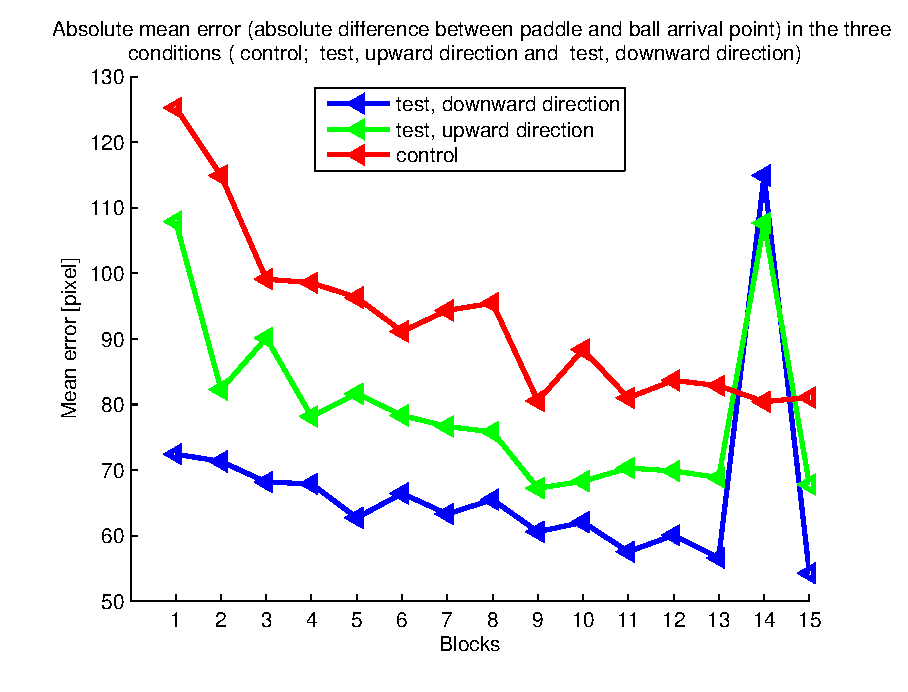
\includegraphics [width=8cm] {fig/TTC.eps}
		\caption{Mean error (difference between paddle and ball arrival point, in absolute value on the right) in the three different conditions (red = control, green = test, upward direction, blue = test, downward direction)}
	\label{figTTC}
\end{figure}

Fig.\ref{figTTC} shows the mean errors for the three conditions and an almost clear separation among all of them can be observed. In all cases there is also an error decrease between the first and the later blocks.
An ANOVA with Condition [two levels: \textit{Test - up} and \textit{Test - down}] as a between-subjects variable, and Block [13 levels. Only the first 13 blocks of trial, in which acceleration was kept constant, were taken into account] as a within-subject variable revealed significant effects of Block [\textit{p-value} $<$ .0001] and of Condition [\textit{p-value} $<$ .0001], corroborating the qualitative observations suggested. The Block $\times$ Condition interaction was not significant [\textit{p-value} $=$ 0.4671].  Consequently there is a significant difference between errors of the two \textit{Test} cases too. In particular subjects who had to deal with  balls affected by a force field whose orientation was opposite to gravity performed constantly worse then the other \textit{Test} group.

\begin{figure}[tb]
	\centering
		\includegraphics [width=15cm] {fig/MultCompTTC.eps}
	\caption{Multiple comparison among marginal means of errors (absolute distance between paddle and ball arrival point) in the three different conditions (from the right: control, test, upward direction and test, downward direction)}
	\label{figMultCompTTC}
\end{figure}

In order to have an overview of the results it is useful to perform a multiple comparison among the means of the errors in the three conditions, which supports the hypothesis of a clear separation between them (see Fig.\ref{figMultCompTTC}).


\textcolor{red}{Observing the error sign in the test groups performances (see Fig.\ref{figTTC}, right panel) it results that subjects at the beginning of the experiment made errors always in the same direction. Who had to deal with trajectories downward oriented usually ended up with the paddle above the real arrival point of the ball, while those who were trying to intercept upward oriented balls missed the catch keeping the paddle below the ball. This could be explained by the hypothesis that during the first blocks of trials subjects try to preview the interception point by interpolating the last part of the ball trajectory with a straight line, tangent to the parabolic curve in correspondence of the beginning of the wall, as described in Fig.\ref{figSchemaRetta}. To check this assumption it has been considered the difference between two distances: the absolute distance between the last paddle position and the real arrival point of the ball ($e_p$) and the absolute distance between the last paddle position and the arrival point of the ball along the presumed tangent straight line ($e_r$). The results, shown in Fig. \ref{figRetta}, suggest that this ``straight line'' strategy is used on the average only during the first sets of blocks, while afterward the prediction seems to become more precise and also tuned to the trajectory parabolic shape.}

\begin{figure}[tbp]
	\centering
		\frame{\includegraphics[width=12cm]{fig/schema_retta.eps}}
		\caption{Scheme of the ball real trajectory and of a possible linear estimate of its last part. In red is depicted the parabolic trajectory, while in green is represented the approximating straight line, corresponding to the curve tangent in the intersection point between the real trajectory and the wall left limit. $e_p$ is the absolute difference between the real arrival point of the ball and the paddle center, while $e_r$ is the absolute difference between the arrival point of the ball along the tangent straight line and the paddle center.}
		\label{figSchemaRetta}
\end{figure}


\begin{figure}[tbp]
	\centering
		\includegraphics[width=15cm]{fig/EsRettaParab.eps}
		\includegraphics[width =8cm]{fig/MediaRettaTmeno.eps}
		\includegraphics[width =8cm]{fig/MediaRettaTpi�.eps}
		\caption{\textbf{Above} - Difference (in pixel) between $e_p$ and $e_r$ for a representative subject. \textbf{Below} - Mean difference (in pixel) between $e_p$ and $e_r$ in each test group: \textbf{Left} - test, downward direction, \textbf{Right} - test, upward  direction. For a definition of $e_p$ and $e_r$ see the caption of Fig \ref{figSchemaRetta}. A positive value of the plot indicates that the paddle at the interception time is nearer to the ball arrival point along the straight line, while a negative value means that the paddle is nearer to the real arrival point of the ball, that follows a parabolic path.}
		\label{figRetta}
\end{figure}



